%%%%%%%%%%%%%%%%%%%%%%%%%%%%%%%%%%%%%%%%%%%%%%%%%%%%%%%%%%%%%%%%%%%%%%%%%%%%%%%%
%2345678901234567890123456789012345678901234567890123456789012345678901234567890
%        1         2         3         4         5         6         7         8


\documentclass[conference]{IEEEtran}
\usepackage{blindtext, graphicx}
\usepackage{listings}
\lstset { %
    language=C++,
    numbers=left,
    breaklines=true,
    xleftmargin=4em,
    resetmargins=true,
    basicstyle=\footnotesize,
    numberstyle=\footnotesize,
}
\usepackage{graphicx}
\usepackage[font=small]{caption}

%Pacote para acentos [Por TIAGO]
\usepackage[utf8]{inputenc}
\usepackage{multirow}
\usepackage{amssymb, amsmath} % Paquetes matemáticos de la American Mathematical Society
\usepackage{float}
\usepackage{multirow}
\usepackage[all]{xy}
\usepackage{tikz}
\usetikzlibrary{matrix}
\usetikzlibrary{calc}
\usetikzlibrary{fit}
%\usepackage{showframe}


% Comment this line out
                                                          % if you need a4paper
%\documentclass[a4paper, 10pt, conference]{ieeeconf}      % Use this line for a4
                                                          % paper

%\IEEEoverridecommandlockouts                              % This command is only
                                                          % needed if you want to
                                                          % use the \thanks command
%\overrideIEEEmargins
% See the \addtolength command later in the file to balance the column lengths
% on the last page of the document



% The following packages can be found on http:\\www.ctan.org
%\usepackage{graphics} % for pdf, bitmapped graphics files
%\usepackage{epsfig} % for postscript graphics files
%\usepackage{mathptmx} % assumes new font selection scheme installed
%\usepackage{times} % assumes new font selection scheme installed
%\usepackage{amsmath} % assumes amsmath package installed
%\usepackage{amssymb}  % assumes amsmath package installed

\title{Comparación de métodos objetivos de evaluación de la calidad del video en videos con diferentes resoluciones espaciales.}

%\author{ \parbox{3 in}{\centering Huibert Kwakernaak*
%         \thanks{*Use the $\backslash$thanks command to put information here}\\
%         Faculty of Electrical Engineering, Mathematics and Computer Science\\
%         University of Twente\\
%         7500 AE Enschede, The Netherlands\\
%         {\tt\small h.kwakernaak@autsubmit.com}}
%         \hspace*{ 0.5 in}
%         \parbox{3 in}{ \centering Pradeep Misra**
%         \thanks{**The footnote marks may be inserted manually}\\
%        Department of Electrical Engineering \\
%         Wright State University\\
%         Dayton, OH 45435, USA\\
%         {\tt\small pmisra@cs.wright.edu}}
%}

% author names and affiliations
% use a multiple column layout for up to three different
% affiliations
\author{
 

\IEEEauthorblockN{Jelena Vlaović, Mario Vranješ, Dominik Grabić, Dregan Samardžija\\}
\IEEEauthorblockA{Faculty of Electrical Engineering, Computer Science and Information Technology Kneza Trpimira 2b, Osijek, Croatia \\ 
Institute RT-RK Osijek LLC Information Technology, Cara Hadrijana 10b, Osijek, Croatia\\
RT-RK Institute for Computer Based Systems, Narodnog Fronta 23a, Novi Sad, Serbia\\
\textsl{jelena.vlaovic@ferit.hr}}
}

\begin{document}

\maketitle
\thispagestyle{empty}
\pagestyle{empty}


%%%%%%%%%%%%%%%%%%%%%%%%%%%%%%%%%%%%%%%%%%%%%%%%%%%%%%%%%%%%%%%%%%%%%%%%%%%%%%%%
\begin{abstract}


A significant progress has been made in adaptive video streaming technology in recent years, but there is still room for improvement using different optimization methods. The goal is to ensure the highest possible video quality perceived by the end users, thus ensuring the highest possible user quality of experience (QoE), regardless of network conditions. Apart from different coding methods, the content itself and the user experience should be considered as optimization parameters. This paper provides a comparison of five objective video quality assessment (VQA) metrics using different video sequences encoded according to H.264/AVC norm at different spatial resolutions and with different target coding bitrates. The metrics included for comparison are Peak Signal-to-Noise Ratio (PSNR), Video Quality Metric (VQM), Structural Similarity index (SSIM), Mean Structural Similarity (MSSIM) index, and Visual Signal-tonoise Ratio (VSNR). The results of the objective VQA metrics have been compared to those of performed subjective VQA experiments. The results show that SSIM and MSSIM achieve the highest performance when evaluating the quality of video sequences of different contents, resolutions and coded with a wide range of coding parameters. Additionally, the results indicate that it is more difficult to efficiently compress the video sequences with higher spatial and temporal activity. Also, due to spatial and temporal masking of compression artifacts in high complexity videos, the analyzed objective VQA metrics achieve lower quality prediction accuracy for that videos.

Keywords- H.264, MSSIM, PSNR, spatial and temporal activity, SSIM, VQM, VSNR

\end{abstract}


%%%%%%%%%%%%%%%%%%%%%%%%%%%%%%%%%%%%%%%%%%%%%%%%%%%%%%%%%%%%%%%%%%%%%%%%%%%%%%%%
\section{Introducción}
    En los últimos años, la transmición de secuencuas de video digital ha invadido todos 
    los segmentos de la vida humana debido a la disponibilidad constante de la conexión a 
    internet y las diferentes aplicaciones de Video on Demand(VoD). En comparación con 
    otros contenidos que se distribuyen a través de Internet, las secuencuas de video siguen 
    siendo las más complejas en términos de adaptación a las condiciones cambiantes de la 
    red y de garantizar la máxima calidad posible para el usuario final.\\
    \\
    Actualmente, las secuencias de vídeo se descargan mediante varios dispositivos 
    con diversas características de haedware y software.\\
    \\
    La transmición adaptativa de secuencias de video ha resuelto muchos problemas 
    adaptación a las condiciones cambiantes de la red, pero aún se están desarrollando 
    nuevos algoritmos de adaptación. La mayoría de los algoritmos de adaptación 
    novedosos se centran en garatizar la máxima calidad de experiencia de usuario 
    (QoE) posible. Para verificar las mejoras realizadas en los algoritmos de transmición 
    adaptativa, se debe probar la calidad de las secuencias de video resultantes. La 
    especificación de calidad de servicio (QoS) depende típicamente del tipo de 
    aplicación para la que se analizan los parámetros. Durante mucho tiempo, la QoS 
    fue el tema dominante de investigación en le dominio de las comunicaciones en red. 
    Surge la pregunta de si los parámetros técnicos de la red satisfacen las necesidades 
    de los usuarios finales.\\
    \\
    Los investigadores de interacción hombre-ordenador (HCI) fueron los primeros 
    en promover el concepto de QoE \cite{biblio1}. Buscaron enfatizar el carácter multidimentsional 
    de la experiencia del usuario y la vitalidad de factores como las emociones, la relación 
    con otras personas, las expectativas y el contexto. Aún así, muchas definiciones de 
    QoE existentes no tienen en cuenta la naturaleza subjetiva de la experiencia del 
    usuario. Por tanto, la QoE se define de muchas formas. Los aurotes en \cite{biblio2} definen 
    QoE como una versión mejorada de Quality of Service (QoS) en el sentido de que 
    QoR brinda información sobre las secuencias de video entregadas desde le punto de 
    vista del usuario final. El UIT-T define QoE como la aceptación subjetiva general de la 
    aplicación o servicio por parte del usuario final \cite{biblio3}. En cualquier definición de QoE, su 
    objetivo es cubrir un área más amplia que solo los parámetros de red. Autores en \cite{biblio4,biblio5}
    han definido QoS como una calidad de la experiencia del usuario que tiene en 
    cuenta todos los aspectos relevantes que definen la satisfacción personal con el 
    servicio. Los autores de \cite{biblio6} afirman que QoE se centra en comprender la calidad 
    general de la experiencia del usuario. Afirman que la QoE es un área multidisciplinar 
    basada en las ciencias de la ingeniería, las ciencias cognitivas, la econimía, la 
    psicología social y la economía.\\
    \\
    Este articulo está estructurado de la siguiente manera: La Sección II ofrece una descripción 
    general del trabaho relacionado con las métricas de calidad objetivas y subjetivas y la influencia de 
    la información espacial y temporal en la calidad de video percibida. La Sección III brinda detalles 
    sobre la configuración de la prueba, las secuencias de video utilizadas, los métodos de codificación 
    y los resultados de la prueba. La Sección III va seguida de una conclusión.



\section{Trabajo relacionado}
    Los métodos utilizados para la evaluación de la calidad de video(VQA) se 
    pueden dividir en métodos objetivos y subjetivos, según la fuente para producir 
    puntuación final de calidad de video distorsionada (computadora o humano, 
    respectivamente). Admás, los métodos objetivos de VQA se dividen en referencia 
    completa (FR), de referencia reducida (RR), y sin referencia (NR), con respecto a los 
    requsitos para el video original al evaluar la calidad del video distorsionado. Los métodos 
    de VQA objetivo de FR se basan generalmente en la medición de las diferencias 
    entre la secuencia de video original y distorcionada, mientras que los métodos 
    de RR requieren solo una serie de características de cada uno de los videos y 
    luego miden la diferencia entre ellos para evaluar la calidad del video 
    distorsionado. Los métodos NR no requieren la información sobre le video 
    original al evaluar la calidad del video distorsionado.\\
    \\
    Los métodos de VQA de objetivo de FR convencionales son, por ejemplo, la 
    relación señal/ruido (SNR), el error cuadrárico medio (MSE), la relación señal/
    ruido pico (PSNR) \cite{biblio7}, el índice de similitud estructiral (SSIM), la similitud estructural 
    media (MSSIM) indice \cite{biblio8}, relación señal/ruido visual(VSNR) \cite{biblio9}, mientras que la 
    métrica RR más utilizada en la literatura es la métrica de calidad de video (VQM) \cite{biblio7}.
    SNR, MSE y PSNR son métricas de VQA basadas en el procesamiento estadistico 
    de diferencias absolutas de píxeles e ignoran las características del Sistema Visual 
    Humano (HVS). Por lo tanto, generalmente no logran aun alta correlación con 
    puntuaciones subjeticas para una amplia gama de parámetros de codificación y 
    transmisión. Se han realizado esfuerzos para desarrollar métricas que se 
    correlacionen mejor con las puntaciones subjeticas de VQA. Se desarrollaron 
    métricas como SSIM y MSSIM en función de las características de HVS. Ambas 
    métricas extraen información estructural de los fotogramas de video y los comparan 
    en lugar de comparar directamente los valores de los píxeles. SSIM se desarrolló 
    teniendo en cuenta que el HVS es muy adecuado para la extracción de información 
    estructural del campo de visión. La distorción visual percibida se estima en SSIM 
    utilizando la distorsión estructural en el video \cite{biblio7}. VSNR es una métrica que 
    considera las propiedades cercanas al umbral y supra-umbral de HVS que se 
    utilizan para cuantificar la preción visual de las secuencias de video. Las 
    propiedades umbral y supre-umbral antes mencionadas se modelan como 
    distancias euclidianas en el espacio de distorción-contraste de descomposición de 
    ondículas multiescala. VSNR se calcula como una suma lineal de las distancias 
    euclidianas antes mencionadas \cite{biblio9}. La métrica VQM basada en la Transformada de 
    coseno discreta (DCT) calcula el nivel de distorsión en secuencias de video 
    codificadas. VQM tiene valor cero si no hubo pérdida durante la compresión y 
    aumenta con el aumento de la degradación de la calidad del video \cite{biblio7}. Es importante 
    tener en cuenta que las pruevas subjetivas brindan la información más precisa sobre 
    el nivel de calidad de la secuencia de video (ya que los humanos. es decir, los 
    usuarios finales evalúan la calidad del video), pero con costosas, complejas y 
    requieren muco tiempo, por lo que, aunque son vitales para el análisis de calidad 
    de secuencias de video, rara vez se realizan.\\
    \\
    El QoS, definida como la prestación de servicios de diferenciación y 
    aseguramiento de la calidad para aplicaciones de internet, generalmetne depende del 
    tipo de aplicación para la que se analizan los parámetros. El problema es que 
    normalmente los parámetros técnicos de la red no cumplen con el final expectaticas de 
    calidad de los usuarios.\\
    Los autores en \cite{biblio10}afirman que el análisis objetivo de la calidad del servicio en la red 
    puede proporcionar información sobre los eventos en la red, por lo que solo 
    proporciona información sobre por qué está sucediendo algo y no cómo ciertos 
    eventos en la red afectan la experiencia del usuario. QoE se centra en la experiencia 
    del usuario y lo que más le afecta.\\
    \\
    Hay muchos factores que influyen y contribuyen a la QoS y QoE al 
    transmitir y repoducir secuencias de video. El procedimiento de 
    procesamiento de secuencias de video consiste en la grabación o generación 
    del video, codificación, compresión, transferencia, decodificación y 
    reproducción. Cada paso del procesamiento de la secuencia de video tiene un 
    impacto directo en la QoE, es decir, la calidad del vídeo puede deteriorarse en cualquiera
    de esos pasos. Medir y optimizar la calidad del video es un problema muy 
    complejo porque deben tenerse en cuenta una amplia variedad 
    de factores técnicos y no técnicos que afectan la calidad de la 
    experiencia de usuario \cite{biblio11}. Los efectos técnicos afectan la calidad 
    del video en términos de irregularidades en la estructura temporal y espacial del 
    video que se introducen en uno de los pasos del procesamiento del video. Del trabajo 
    relacionado, también se puede concluir que los usuarios perciben secuencias de video 
    de aspecto nítido que tienen alto contraste como secuencias de video con mejor 
    calidad de video, en camparación con secuencias de video que tienen bajo 
    contraste, brillo y nitidez \cite{biblio12}.\\
    \\  
    La definición de QoE de ITU-T esteblece que la calidad del video 
    debe evaluarse mediante pruebas subjetivas porque representa el 
    método más preciso para obtener evaluaciones de calidad \cite{biblio13}. En un 
    experimento subjetivo, varios seres humanos están viendo varios 
    videoclips que luego se evalúa en función de lo que han visto y 
    experimentado. El ITU-T propone condiciones de visualización 
    estandar, procedimientos de evaluación, criterios para seleccionar 
    usuarios y materiales y métodos de análisis de datos \cite{biblio14}.\\
    \\
    Según pruebas subjetivas realizadas, los autores de \cite{biblio15}afirman 
    que los eventos de conmutación entre niveles de calidad de video 
    sucesivos perturban la QoE menos que los eventos de conmutación 
    entre los niveles de calidad de video mínimo y máximo. Los autores 
    también concluyeron que si se deteriora la calidad del video del 
    primer segmento temporal, la calidad de la experiencia es menor. El 
    cambio de eventos entre secuencias de video con diferentes 
    resoluciones temporales afecta la QoE menos que el cambio de 
    eventos entre secuencias de video con diferentes resoluciones 
    espaciales. A partir de sus medicions, los autores concluyeron que 
    los resulados de la evaluación subjetiva no siempre pueden 
    correlacionarse  muy bien con los resultados obtenidos de los 
    métodos de prueba objeticos como PSNR.\\
    \\
    Los autores llegaron a la misma conclusión en \cite{biblio16,biblio17}.
    Afirman que es una tarea muy compleja correlacionar los métodos de 
    medición objetiva con el sistema visual humano y que, a veces, el 
    cálculo alto necesario para la métrica del objetivo específico es una 
    pérdida de tiempo computacional. Los autores también han 
    expresado la necesidad de contar con bases de datos más 
    específicas del entorno para mejorar las pruebas de diferentes métricas.\\
    \\
    Aunque los resultados de la evaluación subjetiva no pueden 
    siempre estar altamente correlacionados con los resultados 
    obtenidos de los métodos de prueba objetivos, los autores en \cite{biblio18}
    afirman que las métricas SSIM y local\_PSNR tienen una buena 
    correlación con los resultados de las pruebas subjetivas.\\
    \\
    Aún así, muchos autores indican problemas específicos con respecto
    a las métricas de VQA. De \cite{biblio19} se puede concluir que las pruebas 
    subjetivas pueden verse comprometidas por experiencias previas de 
    los participantes. Los autores de \cite{biblio7}afirman que debería mejorarse la 
    dependencia del contenido de las métricas. Además, los autores de \cite{biblio20} 
    han realizado una observación interesante que debe tenerse en 
    cuenta en el fututo. Afirman que las preferencias de los participantes 
    afectan la evaluación subjetiva de la calidad.

\section{Configuración de prueba y resultados}
    La idea de los experimentos realizados dentro de esta investigación 
    fue comparar el rendimiento de diferentes métricas objetivas de VQA 
    en un conjunto de videos con diferentes características espaciales y 
    temporales (actividades), resoluciones y codificados en diferentes 
    tasas de bits de codificación con las puntuaciones subjeticas. En 
    comparación, se utilizan cinco métricas VQA objetivas (PSNR, SSIM, 
    MSSIM, VQM y VSNR).\\
    \\
    Es importante tener en cuenta que el valir de VQM generalmente 
    disminuye a medida que aumenta la calidad del video, mientras que 
    para todas las demás métricas analizadas, la puntuación de calidad 
    aumenta a medida que aumenta la calidad de video. La idea adicional 
    de los experimentos realizados fue examinar el impacto de la 
    actividad espacial y temporal de las secuencias de video codificadas 
    con tasas de bits de codificación de destino iguales en la calidad de 
    video medida y la experiencia de los usuarios.\\
    \\
    Tres secuencias de video originales en formato YUV sin 
    procesar (YUV420p) del conjunto de datos publicado en \cite{biblio21}. La 
    resolución espacial de estas secuencias es de 1920x1080 píxeles y 
    la velocidad de fotogramas es de 25 fotogramas por sengundo (fps).
    Los nombres de los videos son zonas peatonal (PA), cielo azul (BS) y 
    estación 2 (S2).\\
    \\
    Para medir la actividad temporal y espacial (p. Ej. 
    complejidad) de los videos, la información de percepción temporal 
    (TI) y la información de percepción espacial (SI) se calcularon de 
    acuerdo con \cite{biblio22} para el componente Y de los videos YUV, y los 
    resultados se muestran en la figura \ref{figure1}. Se puede ver que el BS la 
    secuencia de video tiene el mayor SI y TI, mientras que el S2 tiene los 
    valores más bajos. La secuencia de video PA tiene aproximadamente 
    el mismo SI que S2, pero tiene un TI más alto. Se seleccionaron 
    secuencias con diferentes combinaciones de SI-TI para examinar el 
    impacto de SI y TI en una calidad de video medida y percibida. Todas 
    las secuencas de video seleccionadas son filmadas y no generadas 
    por la computadora.\\
    \\
    Programa de línea de comando (CL) de código abierto llamado 
    FFmpeg se usó para codificar secuencias de video usando 
    parámetros de codificación definidos. Todas las secuencias se 
    codificaron según el estándar de compresión de video H.264 / AVC en 
    tres resoluciones espaciales diferentes: nHD (640x360), HD 
    (1280,720), Full HD (1920,1080). Se usó el siguiente comando para 
    codificar secuencias de video en diferentes resoluciones espaciales 
    (el ejemplo se proporciona para la secuencia original S2):\\
    \\
    \textsl{ffmpeg -i station2\_1080p25yuv -c:v libx264 -preset slow- 
        crf 0 -vf scale\=1280x720 station2\_720p25.mp4}
    \\
    Para la codificación de secuencias de video de cada una de las 
    resoluciones, se establecieron diferentes velocidades de bits de 
    codificación de destino. Las tasas de bits de codificación de destino 
    se seleccionaron según la recomendación de los autores de \cite{biblio21}, que 
    seleccionaron las tasas de bits de codifiación de acuerdo con las 
    utilizadas por YouTube. Las tasas de bits de codificación de destino 
    seleccionadas en kbps se enumeran para cada resolución espacial de 
    la siguiente manera:
    
    \begin{itemize}
        \item nHD: 600, 900, 1250, 1600 y 2500 kbps,
        \item HD: 1500, 2500, 4000, y 6000 kbps,
        \item full HD: 2500, 4000, 5000, 6000 y 8000 kbps.
    \end{itemize}

    \begin{figure}[H]
        \centering
        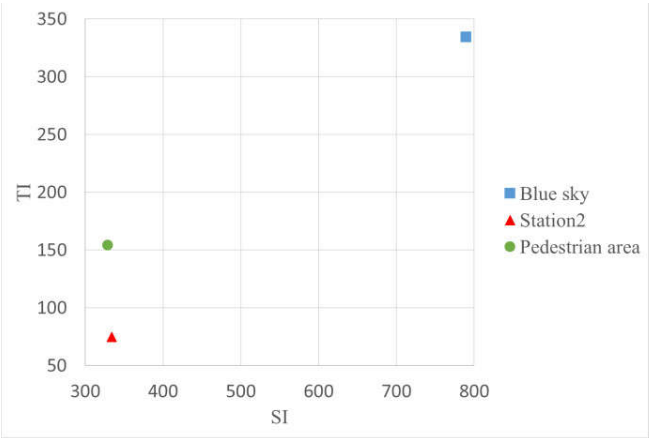
\includegraphics[width=0.4\textwidth]{img/fig1.png}
        \caption{Valores de información de percepción espacial (SI) e información de 
            percepción temporal (TI) para secuencias originales utilizadas en
            experimentos.}
        \label{figure1}
    \end{figure}

    El ajuste preestablecido se establecío en lento ya que era la mejor 
    compensación entre la eficiencia de la compresión y el tiempo 
    requerido para realizar la compresión en sí. El factor de velocidad 
    constante (CRF) es la configuración predeterminada de calidad (y 
    control de velocidad) para el codificador x264 y se estableció en 0 
    para garantizar la mejor calidad posible de la secuencia de video de 
    salida al crear secuencias de video centrales. La codificación 
    posterior se realizó utilizando crf de 23, que es el valor 
    predeterminado en ffmpeg que aún garantiza una buena calidad de 
    video pero también reduce la tasa de bits y el tiempo de codificación.\\
    \\
    El siguiente comando se usó para codificar secuencias de video con 
    diferentes tasas de bits de codificación de destino (el ejemplo se 
    proporciona para la secuencia original S2):\\
    \\ 
    \textsl{ffmpeg -i station2\_1080p25.mp4 -c:v libx264 -x264-params 
    "nal-hrd\=cbr" -b:v 2500k -minrate 2500k -maxrate 2500k bufsize 
    2M-profile:v high -preset slow -crf 23 station2\_1080p25\_2500.mp4}
    \\
    La tasa de bits de codificación lograda difiere ligeramente de las 
    establecidas debido al uso de CRF. La tasa de bits de codificación 
    lograda es, de hecho, la tasa de bits de codificación más baja posible 
    lograda para parámetros de codificación seleccionados en la 
    proximidad de la tasa de bits de codificación objetivos seleccionada.
    Se espera que la tasa de bits de codificación lograda sea mayor para 
    las secuencias con mayor SI y TI, para la misma tasa de bits objetivo 
    establecida durante el proceso de codificación. Parámetros para la 
    codificación de secuencias de vídeo según H.264/AVC: estrategia de 
    codificación general: \textsl{2-pass variable bitrate; profile: high; 
    coding: CABAC entropy coding; level: 4.0; peak rate: 1080p Superbit;} 
    compresión de la curva del cuantificador: 0.9; cuantificación mínima:
    3.\\
    \\
    Antes de evaluar la calidad de los videos codificados por 
    métricas objetivas de VQA, todas las secuencias de video que no 
    tenían una resolución espacial de 1920x1080 píxeles fueron 
    escalas en FFmpeg usando el siguiente comando, con el método 
    de escala de dimensión de Lanczos, de modo que la distorsión de las 
    secuencias de video sería mínima \cite{biblio23}(se proporciona el ejemplo 
    para la secuencia original S2):\\
    \\
    \textsl{ffmpeg -i station2\_720p25.mp4 -vf scale\=1920x1080:flags\=lanczos 
    -c:v libx264 -preset slow -crf 23 station2\_720p25\_upscale.mp4}
    \\
    Dado que las métricas VQA objetivo de FR utilizadas en nuestros 
    experimentos requieren que el video distorsionado tenga la misma 
    resolución espacial que el video de referencia, todas las secuencias 
    de video con una resolución espacial inferior a FullHD se ampliaron a 
    FullHD. Además, la mayoría de los dispositivos de visualización de 
    video actuales tienen pantallas que admiten FullHD y, por lo tanto, 
    tienen SW para escalar las secuencias de video recibidas a una 
    resolución espacial FullHD. Los resultados de las pruebas para todas 
    las métricas objetivas de VQA se calculan procesando el componente 
    Y de los videos YUV. Las Figuras \ref{figure2}-\ref{figure6} muestran los resultados de las 
    pruebas para PSNR, SSIM, MSSIM, VQM y VSNR, respectivamente, 
    para los tres contenidos de video, en las tres resoluciones espaciales 
    seleccionadas y codificadas con diferentes tasas de bits de 
    codificación de destino. En la figura \ref{figure2} se puede ver que los valores de 
    PSNR significativamente más bajos se miden para videos BS que para 
    videos PA y S2. Dichos resultados son la consecuencia de la alta 
    actividad espacial y temporal del video BS, lo que dificulta la 
    codificación de una manera eficiete con parámetros definidos. Si se 
    comparan los valores de PSNR para PA y S2, se puede observar que 
    los valores de PA son ligeramente superiores a los de S2, a pesar de 
    que PA tiene mayor actividad temporal (la actividad espacial es 
    aproximadamente igual para ambos contenidos). Las razones de 
    tales resultados se pueden encontrar en el hecho de que para las 
    mismas tasas de bits de codificación objetivo definidas, las tasas de 
    bits de codificación logradas par las secuencias de PA son 
    ligeramente más altas que las de las secuencias S2 correspondientes, 
    asegurando así probablemente los valores de PSNR ligeramente más 
    altos. Se pueden obtener conclusiones similares a partit de los 
    valores SSIM y MSSIM representados en la figura \ref{figure3} y la figura \ref{figure4}, 
    respectivamente. Tenga en cuenta solo que la diferencia general entre 
    los valores calculados para todas las secuencias de video es menor 
    para SSIM y MSSIM. La razón de esto es la escala que utilizan estas 
    dos métricas (de 0 a 1). De las figuras \ref{figure1}-\ref{figure3}, se puede ver que los valores 
    de PSNR, SSIM y MSSIM aumentan con el aumento de la tasa de bits 
    de codificación lograda, independientemente de SI y TI (como se 
    esperaba). Las diferencias entre esas tres métricas, en términos de 
    percisión de VQA, se mencionan a continuación.\\
    \\
    En la figura \ref{figure5} se presentan los resultados de VQM. Como era de esperar, 
    los valores de VQM disminuyen a medida que aumenta la tasa de bits 
    de codificación lograda y para un contenido de video dado, los valores 
    más bajos de VQM logran secuencias de video con una resolución 
    espacial de 1080p. Debido al hecho de que el contenido de BS tiene la 
    mayor actividad temporal y espacial, es el más difícil de codificar de 
    manera eficiente y, por lo tanto, logra los valores de VQM más altos. 
    La figura \ref{figure6} muesta los resultados de VSNR que en general confirman 
    las observaciones obtenidas al analizar los resultados de otras 
    métricas.

    \begin{figure}[H]
        \centering
        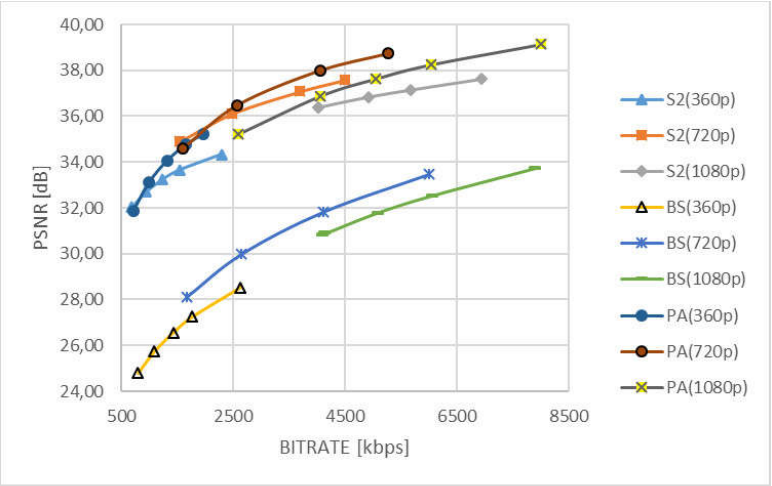
\includegraphics[width=0.4\textwidth]{img/fig2.png}
        \caption{Valores de PSNR para secuencias de vídeo S2, BS y PA codificadas 
        según la norma H.264/AVC utilizando diferentes parámetros de 
        codificación.}
        \label{figure2}
    \end{figure}

    \begin{figure}[H]
        \centering
        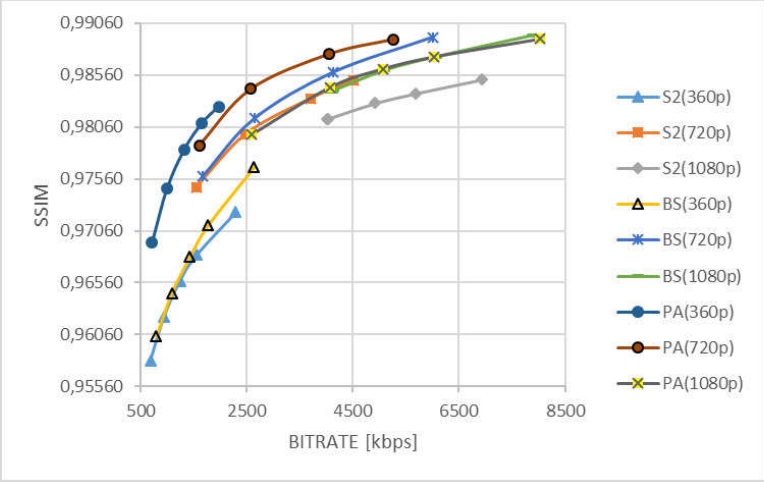
\includegraphics[width=0.4\textwidth]{img/fig3.png}
        \caption{Valores SSIM para secuencias de vídeo S2, BS y PA codificadas de 
        acuerdo con la norma H.264/AVC usando diferentes parámetros de 
        codificación.}
        \label{figure3}
    \end{figure}

    \begin{figure}[H]
        \centering
        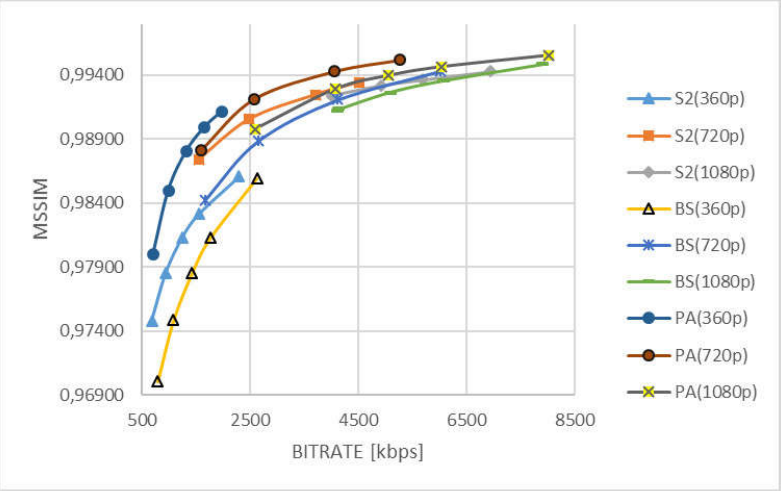
\includegraphics[width=0.4\textwidth]{img/fig4.png}
        \caption{Valores de MSSIM para secuencias de vídeo S2, BS y PA codificadas 
        según la norma H.264/AVC mediante el uso de diferentes parámetros de 
        codificación.}
        \label{figure4}
    \end{figure}

    \begin{figure}[H]
        \centering
        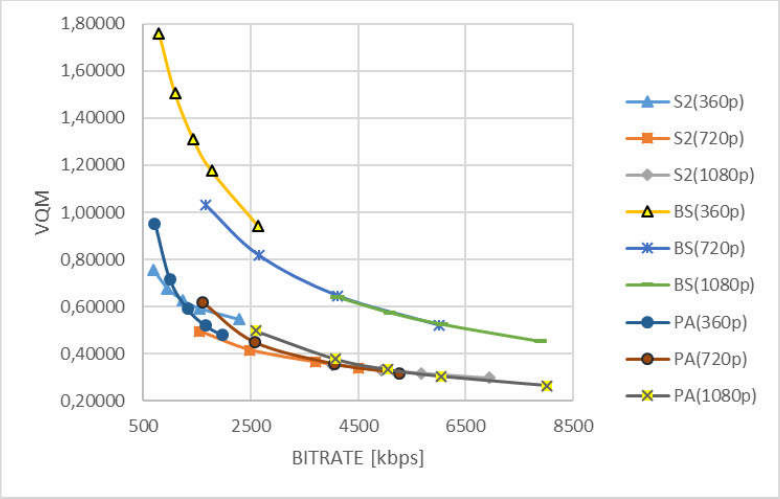
\includegraphics[width=0.4\textwidth]{img/fig5.png}
        \caption{Valores de VQM para secuencias de vídeo S2, BS y PA codificadas 
        según la norma H.264/AVC mediante el uso de diferentes parámetros de 
        codificación.}
        \label{figure5}
    \end{figure}

    \begin{figure}[H]
        \centering
        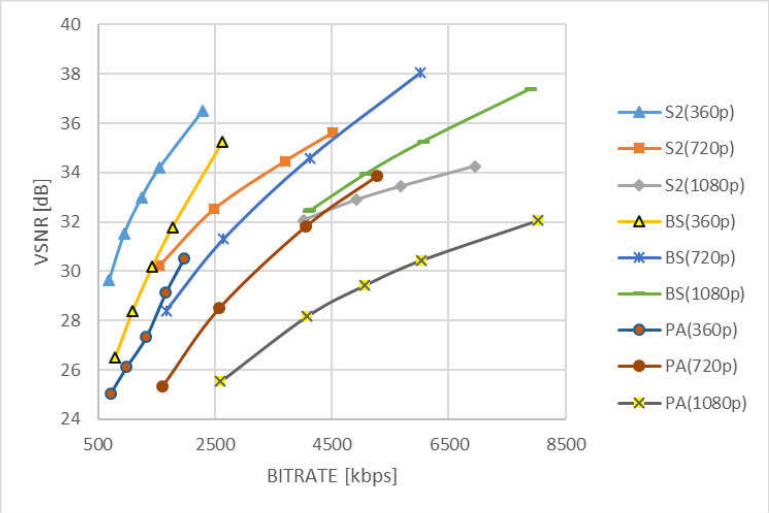
\includegraphics[width=0.4\textwidth]{img/fig6.png}
        \caption{Valores de VSNR para secuencias de vídeo S2, BS y PA codificadas 
        según la norma H.264/AVC mediante el uso de diferentes parámetros de 
        codificación.}
        \label{figure6}
    \end{figure}

    Cuando se compara con los resultados de la métrica PSNR, puede ser 
    visto que los resultados de VSNT indican la mayor diferencia en la 
    calidad de video entre las secuencias del mismo contenido 
    codificadas con diferente tasa de bits de codificación lograda.\\
    \\
    En el análisis adicional proporcionado a continuación, se verificará 
    cuál de esas dos métricas es más precisa, es decir, cuál logra la 
    mayor correlación con las puntuaciones subjetivas de VQA. Para 
    examinar cuál de las cinco métricas analizadas logra el mayor 
    rendimiento en términos de precisión de VQA, los resultados de todas 
    las métricas se comparan con los resultados obtenidos del 
    experimento subjetivo de VQA realizado. En esta invetigación, se 
    realizó un experimento subjetivo de VQA con 26 espectadores sin 
    experiencia en un entorno controlado, como se define en \cite{biblio14}. Hubo 
    13 participantes masculinos y 13 femeninos con edades 
    comprendidas entre los 20 y los 55 años, sin problemas de visión. Se 
    utilizó un muestro no probabilístico para elegir a los participantes. 
    Cada participante vio y evaluó las 45 secuencias de video (42 
    codificadas + 3 secuencias originales). Se utilizan secuencias de 
    video mejoradas en pruebas subjetivas.\\
    \\
    El experimento se realizó en cuatro etapas:

    \begin{itemize}
        \item consentimiento informado: a los participantes  recibieron información 
            básica sobre el experimento,los objetivos del experimento, la agenda, 
            las tareas a realizar y la duración del experimento;
        \item preselección de sujetos: se han realizado una prueba de agudeza 
            visual y una prueba de visión cromática de Ishihara para detectar 
            deficiencias visuales; 
        \item instrucciones y capacitación: los participantes recibieron 
            instrucciones detalladas sobre cómo evaluar las secuencias de video 
            y se familiarizaron con los mejores y peores escenarios de todas las 
            secuencias de video;
        \item sesión de votación: se realizó mediante sesiones de 
            ritmo fijo con diez para la votación que se realizó en 
            boletas de papel;
    \end{itemize} 

    La puntuación media de opinión (MOS) de cada vídeo evaluado fue 
    calculado como un valor medio de los resultados obtenidos de todos 
    los sujetos para una determinada secuencia de vídeo visualizada. 
    Para medir la correlación entre los puntajes subjetivos y las 
    puntuaciones de una métrica VQA objetiva particular, se calculó el 
    coeficiente de correlación lineal de Pearson (PLCC) \cite{biblio24}. Los 
    resultdos de PLCC se han calculado para cada contenido por 
    separado utilizando todos los resultados adquiridos para ese 
    contenido (todas las resoluciones espaciales y todas las tasas de bits 
    de codificación de destino), así como para las 45 secuencias juntas. 
    Los resultados de PLCC se dan en la Tabla \ref{Tabla1}.\\
    \\
    Al analizar los resultados logrados por diferentes métricas para un 
    contenido de video en particular, se puede ver que para cada 
    contenido, otra métrica logra el mejor resultado, es decir, VQM para 
    S2, VSNR para BS, PSNR para PA. Por otro lado, cada una de estas 
    métricas que logran el PLCC más alto para uno de los contenidos, 
    logra resultados bastante pobres para algunos de los otros 
    contenidos o para todos los contenidos juntos, donde VQM, VSNR y 
    PSNR logran un PLCC más bajo que SSIM y MSSIM. Aunque SSIM y 
    MSSIM no logran el mayor rendimiento para ningún contenido en 
    particular, logran el mayor rendimiento al analizar los resultados de 
    todas las secuencias juntas. Por tanto, se puede concluir que SSIM 
    y MSSIM son la mejor opción para evaluar la calidad de secuencias de 
    video de diferentes contenidos, resoluciones y codificadas con una 
    amplia gama de parámetros de codificación. Dado que tienen en 
    cuenta las características de HVS, superan significativamente a PSNR 
    y VSNR.\\
    \\
    Además, se puede ver que cada métrica, excepto VSNR, logra el PLCC 
    más bajo para el contenido de video B2, que tiene la mayor actividad 
    espacial y temporal. Un análisis más profunco de los resultados 
    experimentales mostró que la menor correlación para el contenido de 
    video de B2 lograda por la métrica analizadas generalmente es 
    causada por el enmascaramiento espacial y temporal de los errores 
    que ocurren en las secuencias de video de B2. Es decir, las 
    deficiencias introducidas en los videos B2 en el proceso de 
    codificación son menos visibles para los espectadores debido a la 
    gran cantidad de detalles y movimientos rápidos en el video.\\
    
    \begin{table}
        \begin{center}
            \begin{tabular}{| r | l | c |}
                \hline
                \textbf{Métrica objetiva} & \textbf{Contenido de video} & \textbf{PLCC} \\ \hline
                \multirow{4}{1.5cm}{PSNR} & S2 & 0,928356 \\ \cline{2-3}
                    & BS & 0,889061 \\ \cline{2-3} 
                    & PA & 0,966959 \\ \cline{2-3} 
                    & Todas las secuencias & 0,649198 \\ \hline
                \multirow{4}{1.5cm}{SSIM} & S2 & 0,922531 \\ \cline{2-3}
                    & BS & 0,86543 \\ \cline{2-3} 
                    & PA & 0,9423499 \\ \cline{2-3} 
                    & Todas las secuencias & 0,837148 \\ \hline
                \multirow{4}{1.5cm}{MSSIM} & S2 & 0,871447 \\ \cline{2-3}
                    & BS & 0,870457 \\ \cline{2-3} 
                    & PA & 0,932319 \\ \cline{2-3} 
                    & Todas las secuencias & 0,835342 \\ \hline
                \multirow{4}{1.5cm}{VQM} & S2 & 0,93671 \\ \cline{2-3}
                    & BS & 0,87557 \\ \cline{2-3} 
                    & PA & 0,95345 \\ \cline{2-3} 
                    & Todas las secuencias & 0,67315 \\ \hline
                \multirow{4}{1.5cm}{VSNR} & S2 & 0,177292 \\ \cline{2-3}
                    & BS & 0,938999 \\ \cline{2-3} 
                    & PA & 0,725848 \\ \hline
                \textbf{Métrica objetiva} & \textbf{Contenido de video} & \textbf{PLCC} \\ \hline
                    & Todas las secuencias & 0,409926 \\ \hline
            \end{tabular}
            \caption{Resultados de correlación lineal de Pearson.}
            \label{Tabla1}
        \end{center}
    \end{table}

    Por otro lado, la métricas analizadas, que no incorporan efectos de 
    enmascaramiento espacial y temporal en sus algoritmos, sobreestiman 
    las deficiencias visibles y producen puntuaciones de calidad inferiores 
    a las obtenidas por humanos. En consecuencia, la correlación para el 
    contenido de video BS es menor que para otros contenidos. 

\section{Concluciones}
    En la última década se han desarrollado diferentes aplicaciones 
    multimedia, principalmente aplicaciones de transmisión de video.
    Varios métodos de codificación, la percepción del usuario de la 
    calidad del vídeo y la influencia de la actividad espacial y temporal del 
    contenido deben tenerse en cuenta como parámetros de optimización 
    en tales aplicaciones. Debido al hecho de que las pruebas subjetivas 
    son costosas y requeren mucho tiempo, se utilizan métricas 
    objetivas de VQA para evaluar la calidad de las secuencias de video 
    codificadas. En este documento, se comparan cinco métricas 
    objetivas de VQA en términos se precisión de evaluación de calidad 
    de video. La correlación con los resultados de los experimentos 
    subjetivos se calcula para cada métrica objetiva de VQA. Los 
    resultados muestran que SSIM y MSSIM logran el mayor rendimiento 
    al evaluar la calidad de secuencias de video de diferentes contenidos, 
    resoluciones y codificadas con una amplia gama de parámetros de 
    codificación. Además, los resultados indican que es más difícil 
    comprimir de manera eficiente las secuencias de video con mayor 
    actividad espacial y temporal que aquellas con menor actividad. 
    Además, debido al enmascaramiento espacial y temporal de los 
    artefactos de compresión en videos de alta complejidad, las métricas 
    analizadas logran la precisión de predicción de la más baja calidad 
    para esos videos. En el trabajo futuro, se analizará el mayor número 
    de contenidos de video diferentes y se tomarán en consideración 
    métricas de VQA objetivas adicionales porque tres contenidos de 
    video diferentes son suficientes para obtener conclusiones generales. 
    A partir del análisis extendido, la idea final de nuestro trabajo futuro 
    es proponer una nueva métrica objetiva de VQA que logrará una 
    correlación con puntuaciones subjetivas superiores a todas las 
    métricas analizadas.

\section{Reconocimiento}
    ESte trabajo fue parcialmente apoyado por J.J. Strossmayer fondo 
    empresarial de la Universidad de Osijek a través del concurso interno 
    para los proyectos artísticos y de investigación "UNIOS ZUP-2018" y 
    parcialmente por el Ministerio de Educación, Ciencia y Desarrollo 
    Tecnológico de la Republica de Serbia, con el número de concesión 
    TR36029.

\begin{thebibliography}{99}
    \bibitem{biblio1}
        Y. Chen, K. Wu, and Q. Zhang, “From QoS to QoE: A tutorial on 
        video quality assessment,” IEEE Communications Surveys \& Tutorials, 
        vol. 17, pp. 1126 1165, October 2015. 
    \bibitem{biblio2}
        S. R. Lima and P. Carvalho, “Enabling self adaptive QoE / QoS 
        control, ” 36th Conference on Local Computer Networks, pp. 239 242, 
        October 2011
    \bibitem{biblio3}
       “ITU T G.1080 Quality of experience requirements for IPTV services,” 
       International Telecommunication Union, pp. 1 44, 2008.
    \bibitem{biblio4}
       J. M. G. Stensen, “Evaluating QoS and QoE Dimensions in Adaptive 
       Video Streaming,” Institutt for telematikk, pp. 21 34, June 2012.
    \bibitem{biblio5}
       J. P. Hansen and S. A. Hissam, “Assessing QoS tradeoffs for real-time 
       video,” 14th International Symposium on "A World of Wireless, Mobile 
       and Multimedia Networks" (WoWMoM), pp. 1-6, June 2013.
    \bibitem{biblio6}
       G. Pibiri, C. Mc Goldrick, and M. Huggard, “Expected Quality of Service 
       (eQoS) A network metric for capturing end-user experience,” IFIP Wirel. 
       Days, November 2012.
    \bibitem{biblio7}
       M. Vranješ, S. Rimac-Drlje, D. Žagar, “Objective Video Quality Metrics”, 
       49th International Symposium ELMAR, pp. 45-49, September 2007.
    \bibitem{biblio8}
        C. Yang, L. Zhao and Z. Liao, "Objective Quality Metric Based on 
        Perception for Video," International Conference on Computer Engineering and 
        Technology, pp. 20-33, January 2009. 
    \bibitem{biblio9}
        D. M. Chandler and S. S. Hemami, "VSNR: A wavelet-based visual signal-to-noise 
        ratio for natural images", IEEE Transactions on Image Processing, vol. 16, 
        pp. 2284-2298, August 2007.
    \bibitem{biblio10}
        P. Orosz, T. Skopkó, Z. Nagy, P. Varga, and L. Gyimóthi, “A case study on 
        correlating video QoS and QoE,” IEEE Network Operations and Management Symposium 
        (NOMS), pp. 1-5, May 2014.
    \bibitem{biblio11}
        V. Deksnys, E. Sakalauskas and G. Činčikas, “New integral quality of TV service 
        criterion construction based on quality of experience statistical estimation,” 
        14th Biennial Baltic Electronic Conference (BEC), pp. 149–152, October 2014.       
    \bibitem{biblio12}
        R. Koshimura, Y. Ito and Y. Nomura, “Empirical study on clarification of relationship 
        between QoS and QoE for Web services by path analysis,” 3rd Global Conference on 
        Consumer Electronics (GCCE), pp. 10-11, 2014, October 2014.
    \bibitem{biblio13}
        “ITU-T P.10 Vocabulary for performance, quality of service and quality of 
        experience.”, International Telecommunication Union, pp. 1-22, 2017.
    \bibitem{biblio14}
        “ITU-T P.912: Subjective video quality assessment methods for recognition tasks.”, 
        International Telecommunication Union, pp. 1-22, 2016.
    \bibitem{biblio15}
        T. Zinner, O. Hohlfeld, Osama Abboud and T. Hossfeld, “Impact of Frame Rate and 
        Resolution on Objective QoE Metrics,” Second International Workshop on Quality 
        of Multimedia Experience (QoMEX), pp. 29-34, June 2010.
    \bibitem{biblio16}
        R. Singh and N. Aggarwal, “State of the Art and Research Issues in Video Quality 
        Assessment,” RAECS UIET Panjab University Chandigarh, pp. 1-6, March 2014.
    \bibitem{biblio17}
        Nidhi and N. Aggarwal, “A Review on Video Quality Assessment”, RAECS UIET Panjab 
        University Chandigarh, pp. 1-6, March 2014.
    \bibitem{biblio18}
        M. Vranješ, S. Rimac-Drlje, D. Žagar, “Subjective and Objective Quality Evaluation 
        of the H.264/AVC Coded Video,” 15th International Conference on Systems, Signals and 
        Image Processing, pp. 287 – 290, June 2008.
    \bibitem{biblio19}
        P. Orosz, T. Skopkó, Z. Nagy, P. Varga and L. Gyimóthi, “A Case Study on Correlating 
        Video QoS and QoE,” IEEE Network Operations and Management Symposium (NOMS), pp 1-5, May 
        2014.
    \bibitem{biblio20}
        D. Z. Rodríguez, R. L. Rosa, E. A. Costa, J. Abrahão, and G. Bressan, “Video Quality Assessment 
        in Video Streaming Services Considering User Preference for Video Content,” IEEE 
        Transactions on Consumer Electronics, vol. 60, pp. 570 - 571, March 2014.
    \bibitem{biblio21}
        C. Kreuzberger, D. Posch, and H. Hellwagner, “A Scalable Video Coding Dataset and 
        Toolchain for Dynamic Adaptive Streaming over HTTP,” 6th ACM Multimedia Systems 
        Conference, pp. 213-218, March 2015.
    \bibitem{biblio22}
        “ITU-T P.911 Subjective audiovisual quality assessment methods for multimedia 
        applications,” International Telecommunication Union, pp. 1-27, 1998.
    \bibitem{biblio23}
        J. Chen and Y. Saad, “Lanczos Vectors versus Singular Vectors for Effective Dimension 
        Reduction”, IEEE Transactions on Knowledge and Data Engineering, vol. 21, pp. 1091-1103, 
        November 2009.
    \bibitem{biblio24}
        M. Vranješ, S. Rimac-Drlje and K. Grgić, “Locally averaged PSNR as a simple objective Video 
        Quality Metric”, 50th International Symposium ELMAR, vol 1, pp. 17-20, September 2008.

    \end{thebibliography}

\end{document}
